\documentclass{beamer}

\usepackage{beamerthemesplit}
\usetheme{Warsaw}
\setbeamertemplate{navigation symbols}{}
\setbeamercovered{transparent=25}

\title{An Overview of Complex Networks Design and Analyses}
\author[Sanket Patil]{Sanket Patil}

%\institute{
%\textbf{Advisor}: Dr. Srinath Srinivasa\\
%Open Systems Laboratory \\ 
%			International Institute of Information Technology\\
%			Bangalore\\
%			India		
%			
%			}

%\date[OT]{International Conference on Intelligent Systems - 2005\\December 3, 2005}

\begin{document}

\frame {\titlepage}

\section[Outline]{}
	\frame{\tableofcontents}

\section{Introduction}
	\subsection{Definition}
	\frame
				{
				\frametitle{Complex Networks}
				\begin{itemize}
					\item<1-> {Not ``simple networks''}
					\item<2-> {Not random graphs}
					\item<3-> {Have non-trivial topological features}
				\end{itemize}				
				}
				
			

		\frame
			{
			\frametitle{Examples}
			\begin{itemize}
				\item<1-> {Computer Networks, the Internet, the Web}
				
				\item<2-> {Food-webs, protein interaction networks}
				
				\item<3-> {Social Networks, Trade Networks}
				
				\item<4-> {The brain}
			\end{itemize}
			}
		
		\frame
		{
			\frametitle{Complex Networks}
			\begin{itemize}
				\item<1-> {Designed (for performance)}
				\item<2-> {Have evolved/emerged over time}
				\item<3-> {Are teleological / have purpose of life}
			\end{itemize}
		}
	\subsection{Representation}		
				\frame
				{
					\frametitle{Representation}
					\begin{itemize}			
						\item<1-> {Networks are modelled as ``Graphs''}
						\item<1-> {A node/vertex/point represents a machine, a human, a cell etc.}
						\item<1-> {An edge/arc/line represents a \textit{relation} between two nodes}
						\item<1-> {Edges can be undirected or directed.}
						\item<1-> {\textit{Weights} are used to convey additional (extra-topological) information}
					\end{itemize}
						
				}

				\frame
				{
					\frametitle{Basic Definitions}
					\begin{itemize}
						\item<1-> {\textbf{Degree:} The number of edges \textit{incident} on a node}
						\item<1-> {\textbf{Indegree (outdegree):} Number of incoming (outgoing) edges}
						\item<2-> {\textbf{Degree Distribution:} A probability distribution of node degrees}
					\end{itemize}
				}
			
				\frame
				{
					\begin{itemize}
					\item<1-> {\textbf{Path:} A sequence of \textit{adjacent} vertices}
					\item<1-> {\textbf{Pathlength:} The number of edges in a path}
					\end{itemize}
				
					\begin{centering}			
					\begin{figure}
						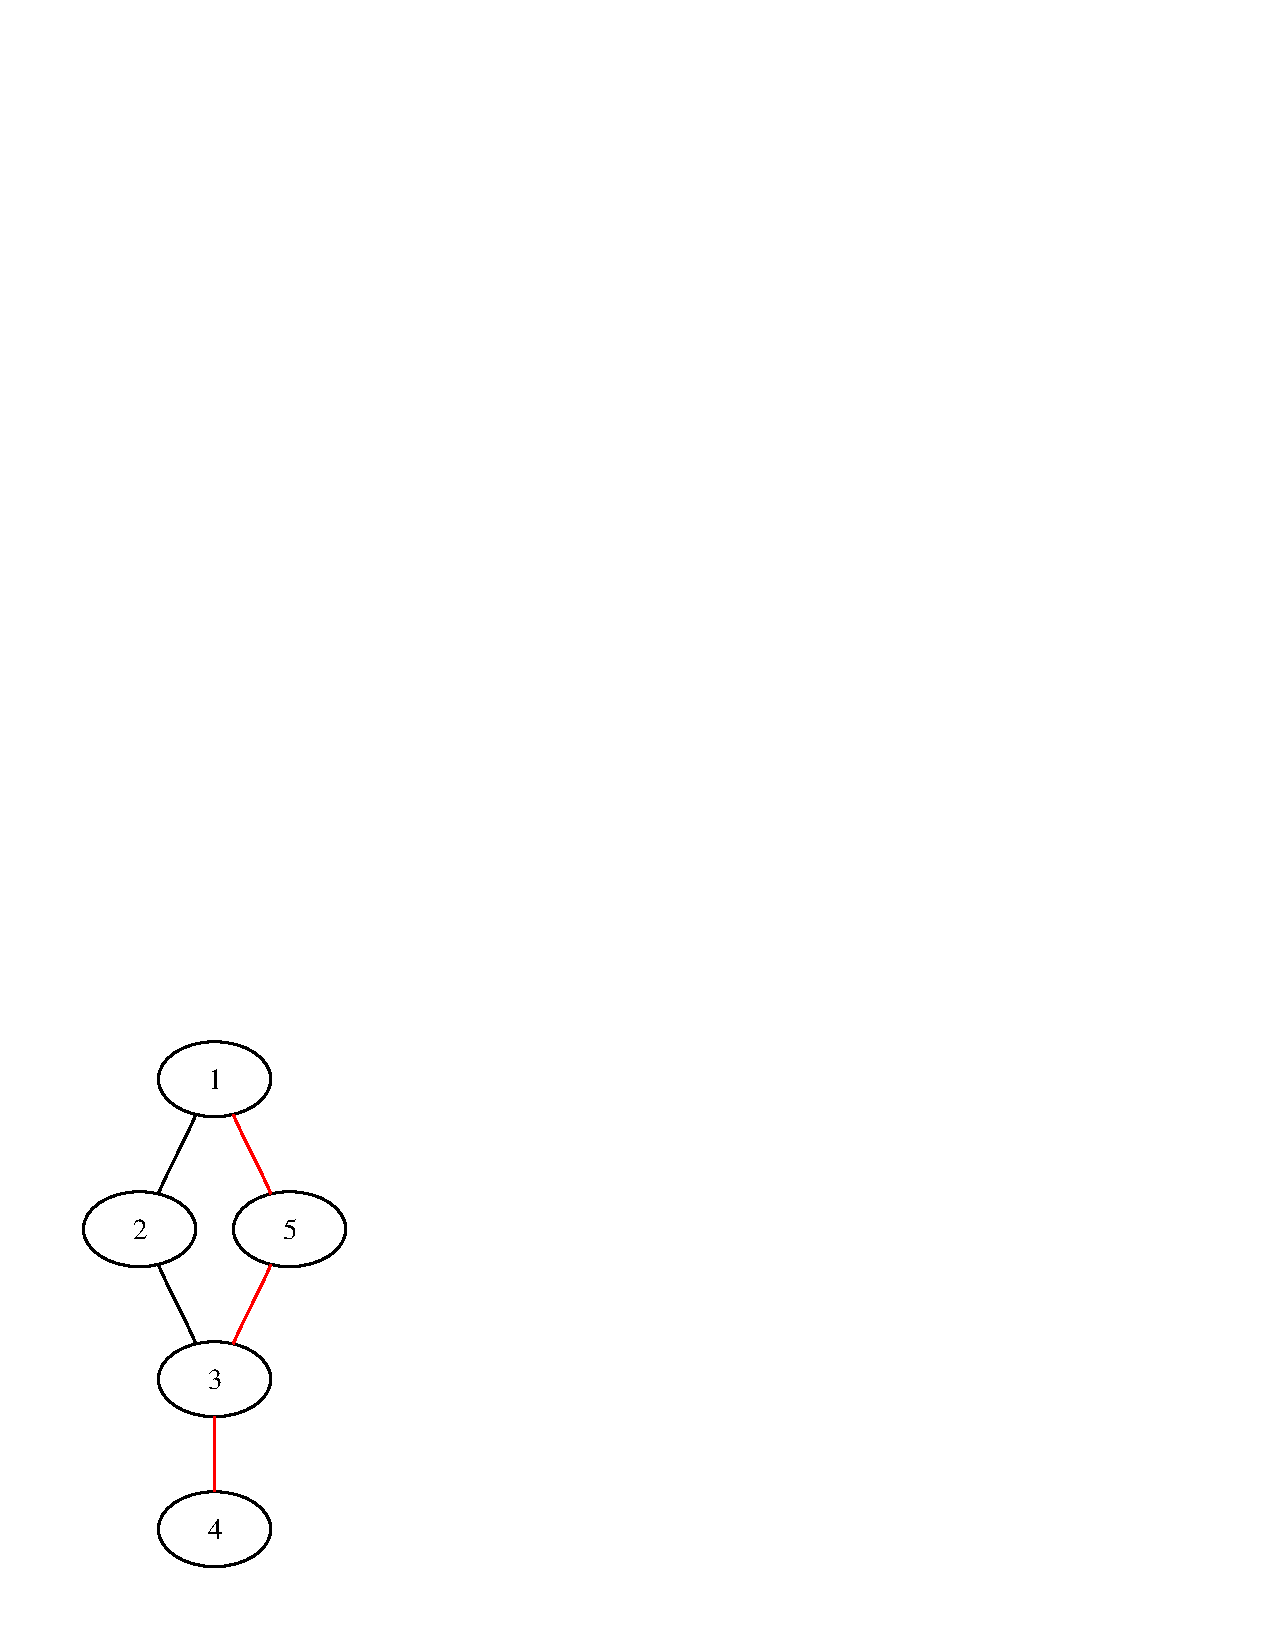
\includegraphics[height=2in]{graph.jpg}
					\end{figure}
					\end{centering}					
					
				}

\section{Topological Features}
	\subsection{Scale-free Nature}
		\frame
		{
			\frametitle{Scale-free Nature}
				\begin{itemize}
					\item<1-> {Network dynamics/behaviour is independent of the size}
					\item<2-> {Power Law degree distributions} 
				\end{itemize}
		}
		\frame
		{
			\frametitle{Power Law Distribution}
			\begin{centering}			
			\begin{figure}
				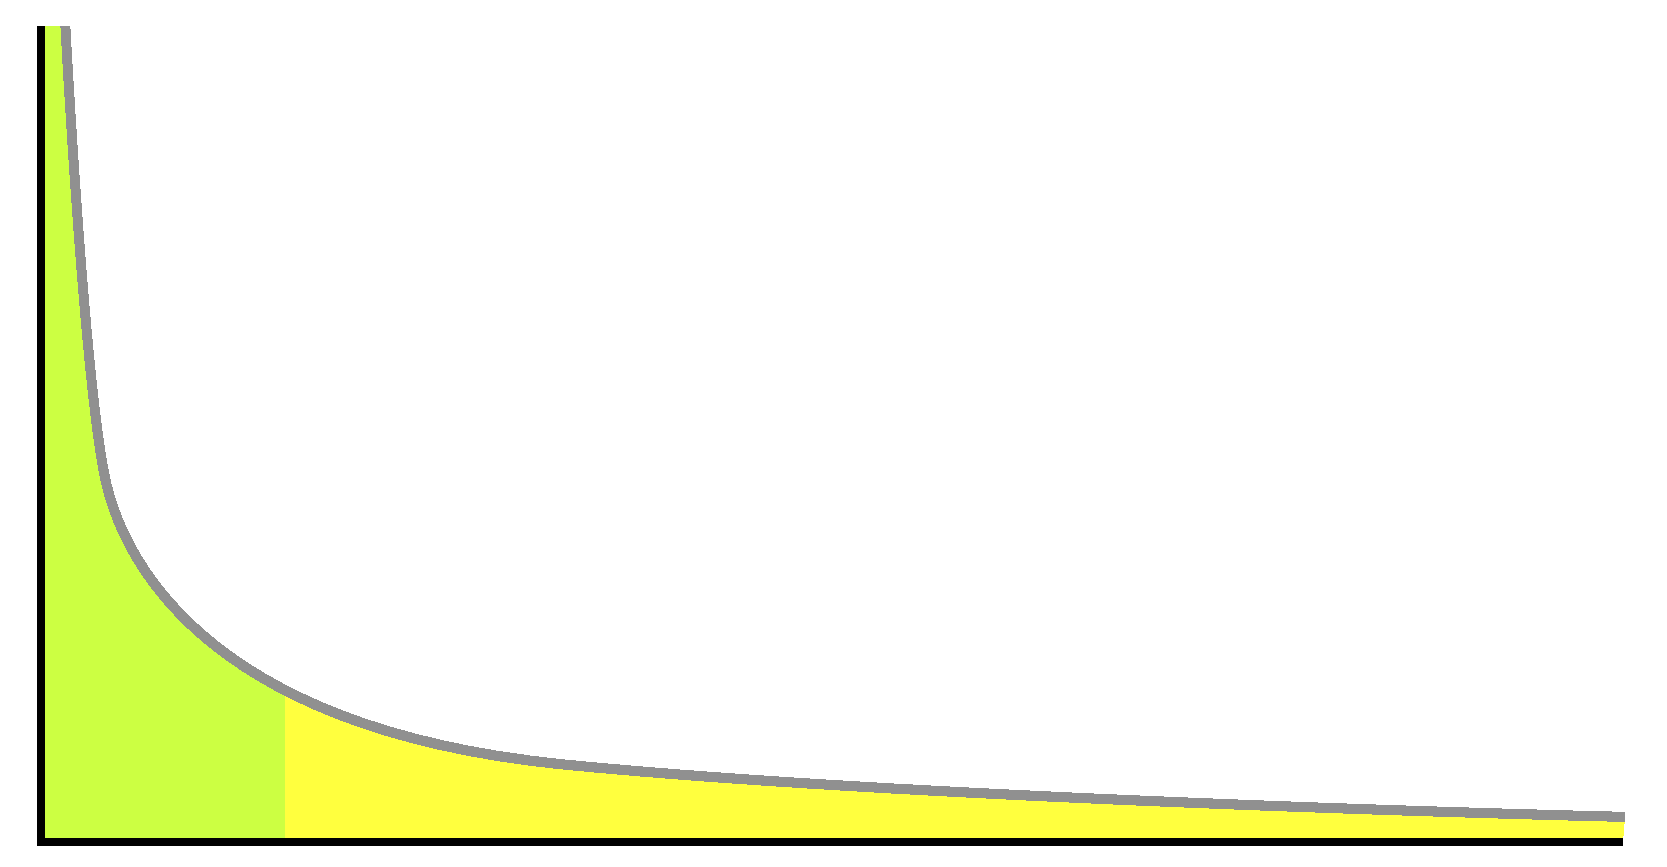
\includegraphics[height=2in]{Long_tail}
			\end{figure}
			\end{centering}					
					
		}
		\frame
		{
			\frametitle{Properties}
			\begin{itemize}
				\item<1-> {$P[X=k] \  \alpha \  k^{-p}$ }
				\item<2-> {Small number of nodes with a very high degree and a large number of nodes with a very low degree}
				\item<3-> {``heavy tail'', ``long tail'', ``80:20''}
				\item<4-> {Income distributions, page rank, wikipedia contribution}
			\end{itemize}
		}
		\frame{
		\frametitle{Preferential Attachment}
			\begin{itemize}
			\item<1-> {Nodes prefer to attach to ``popular'' nodes}
			\item<2-> {``Rich getting richer''}
			\item<3-> {Entrenchment}
			\end{itemize}	
		}
	\subsection{``Small World'' properties}
		\frame
		{
			\frametitle{``Small World'' Properties}
				\begin{itemize}
					\item<1-> {Stanley Milgram: Small world experiment}
					\item<2-> {Mean Path Length ~ 6}
					\item<3-> {Critique: not a comprehensive study}
					\item<4-> {``Six degrees of separation''}
					\item<5-> {Watts and Strogatz}
				\end{itemize}
		}
		\frame
		{
			\frametitle{Saul Steinberg: Ninth Avenue}
			\begin{centering}			
			\begin{figure}
				\includegraphics[height=2.25in]{newyorker2.jpg}
			\end{figure}
			\end{centering}					
		}
		\frame
		{
			\begin{itemize}
				\item<1-> {Social Commentary}
				\item<2-> {Small world geometry}
			\end{itemize}
		}
		
		\frame	
		{
			\frametitle{Kleinberg's ``small world''}
				\begin{itemize}
					\item<1-> {Ninth Avenue as a powerful analogy}
					\item<2-> {The ``far'' is almost as accessible as the ``near''}
					\item<3-> {How are your friends/acquaintances distributed?}	
				\end{itemize}
		}
		
		\frame
		{
			\frametitle{Clustering}
			\begin{centering}			
			\begin{figure}
				\includegraphics[height=2.25in]{cluster.jpg}
			\end{figure}
			\end{centering}						
		}
		\frame
		{
			\frametitle{Clustering Coefficient}
				\begin{itemize}
					\item<1-> {\textbf{Neighbourhood:} Nodes that are adjacent to a node}
					\item<2-> {$C_{i} = \frac{no\ of\ edges\ in\ the\ neighbourhood}{total\ possible\ edges}$}
					\item<3-> {$C_{graph} = \frac{\sum_{i=0}^n C_{i}}{n}$}
				\end{itemize}
		}
		\frame
		{
			\frametitle{Small Worlds}
				\begin{itemize}
					\item<1-> {High clustering coefficient}
					\item<1-> {Low average path length}
				\end{itemize}
		}
		\frame
		{
			\frametitle{Navigability in small worlds}
				\begin{itemize}
				\item<1-> {Kleinberg's metric space models (circa 2000)}
				\item<2-> {Short paths do exist}
				\item<3-> {But can we \textit{find} them using \textit{local} information?}	
				\end{itemize}
		}
		\frame
		{
			\frametitle{Short range and long range connections}
			\begin{centering}			
			\begin{figure}
				\includegraphics[height=2.25in]{grid.jpg}
			\end{figure}
			\end{centering}
		}
		\frame
		{
			\frametitle{Clustering Exponent}
				\begin{itemize}
					\item<1-> {Connections based on distance (r) and clustering exponent $\alpha$}
					\item<2-> {For a node $u$, the probability of connecting to $v$ is $r^{-\alpha}$}
					\item<3-> {Highly clustered neighbourhood}
					\item<4-> {Number of long range links decays with distance}
					\item<5-> {Only when $\alpha = 2$, a decentralized routing algorithm can be found which has a $log\ n$ bound}
				\end{itemize}	
		}

		\frame
		{
			\frametitle{Finding short paths}
			\begin{centering}			
			\begin{figure}
				\includegraphics[height=2.25in]{short-paths.jpg}
			\end{figure}
			\end{centering}

		}

	\subsection{Other features}
		\frame
		{
			\frametitle{Other Features}
				\begin{itemize}
					\item<1-> {Communities}
					\item<2-> {Hierarchical Structures}
				\end{itemize}
		}

	\section{Philosophy}
	\frame
	{
		\frametitle{Complex Systems: Philosophy}
			\begin{itemize}
				\item<1-> {Systems Theory}
				\item<2-> {Cybernetics}
				\item<3-> {Non-linear Dynamics}
				\item<4-> {Multiagent Systems and AI}
				\item<5-> {Network Science, Connectionism, Cognitive Psychology}
			\end{itemize}
	}

	\frame
	{
		\frametitle{Strudy of Complex Networks}
			\begin{itemize}
				\item<1-> {Structure or Topology}
				\item<2-> {How structure governs the function}
				\item<3-> {How design can be analysed teleologically}
				\item<4-> {Can we use this knowledge to build better systems?}
			\end{itemize}
	}

	\subsection{Emergence}
		\frame
		{
			\frametitle{Emergence}
			\begin{itemize}
				\item<1-> {The connections between the components is as important as the components}
				\item<2-> {Emergent behaviour of complex networks}
				\item<3-> {Case Study: The Human Brain}
			\end{itemize}
		}

	\subsection{Machines vs Societies}
		\frame
		{
			\frametitle{Machines vs Societies}
				\begin{itemize}
					\item<1-> {Systems Thinking: parts and whole}
					\item<2-> {Machines funcion based on norms}
					\item<3-> {Societies are declarative}
					\item<4-> {Societies are more robust}
					\item<5-> {Case study: The Heart}
				\end{itemize}
		}

	\subsection{Self Interest}
		\frame
		{
			\frametitle{Self Interest}
				\begin{itemize}
					\item<1-> {Autonomous agents}
					\item<2-> {Local constraints and self interest}
					\item<3-> {Global or environmental dampeners}
				\end{itemize}
		}
	
\section{Design}
	\subsection{Systems Design: Desiderata}
	\frame
	{
		\frametitle{Systems Design: Desiderata}
		\begin{itemize}
			\item<1-> {Safety}
			\item<2-> {Resilience}
			\item<3-> {Fairness}
			\item<4-> {Livenss}
		\end{itemize}
	}

\subsection{Complex Systems Design}
	\frame
	{
		\frametitle{Complex Systems Design}
		\begin{itemize}
			\item<1-> {Efficiency}
			\item<2-> {Robustness}
			\item<3-> {Cost}
		\end{itemize}
	}


	\frame
	{
		\frametitle{An Optimization Problem}
			\begin{itemize}
				\item<1-> {Designing complex systems is an optmization process}
				\item<2-> {Search in a multidimensional space}
			\end{itemize}
	}

	\frame
	{
		\frametitle{Approaches}
			\begin{itemize}
				\item<1-> {Mathematical Programming}
				\item<1-> {Ant Colony Optimization}
				\item<1-> {Swarm Intelligence}
				\item<1-> {Simulated Annealing}
				\item<1-> {Genetic Algorithms}
			\end{itemize}
	}

\section{Analyses}
	\frame
	{
		\frametitle{Graph Theoretic Analyses}
			\begin{itemize}
				\item<1-> {Graph thoretic properties used in design and analyses}
				\item<2-> {Constraints and objectives are defined in terms of graph properties}
				\item<3-> {Design is usually evolution of optimal graphs under the given constraints}
			\end{itemize}
	}

	\frame
	{
		\frametitle{Efficiency}
			\begin{itemize}
				\item<1-> {\textbf{APL:} Average of all pairs shortest paths}
				\item<2-> {\textbf{Diameter:} The longest shortest path. An upper bound on efficiency.}				
			\end{itemize}
		
	}	

	\frame
	{
		\frametitle{Local Objectives}
		\begin{itemize}
			\item<1-> {\textbf{Eccentricity: } The longest shortest path \textit{for a node}}
			\item<2-> {The greatest separation a node suffers}
			\item<3-> {Average eccentricity or eccentricity distribution are also good indicators of efficiency}
			\item<4-> {\textbf{Radius:} Smallest eccentricity. ``Central'' node}
			\item<5-> {Number of ``central'' nodes can be another measure}
		\end{itemize}
	}
%$\frac{no\ of\ edges\ in\ graph}{n(n - 1)}}$
\frame
	{
		\frametitle{Cost}
			\begin{itemize}
				\item<1-> {\textbf{Density(connectance): no of edges/no of possible edges} }
				\item<2-> {Edges per node}
				\item<3-> {Weights, costs and other environment dependent measures}
			\end{itemize}
	}

	\frame
	{
		\frametitle{Robustness}
			\begin{itemize}
				\item<1-> {Centrality Measures}
				\item<2-> {Connectivity}
			\end{itemize}
	}

	\frame
	{
		\frametitle{Centrality}
			\begin{itemize}
				\item<1-> {\textbf{Degree Centrality:} degree distribution}
				\item<2-> {\textbf{Betweenness:} importance of nodes based on the no. of paths passing through them}
				\item<3-> {\textbf{Closeness:} \textit{per node} average path length}
				\item<4-> {\textbf{Eigenvector Centrality:} importance of nodes based not just on \textit{how many} are endorsing, but also \textit{who} is connected.}
				\item<5-> {When a centrality distribution is uniform, the network is most robust}
			\end{itemize}
	}

	\frame
	{
		\frametitle{Connectivity}
			\begin{itemize}
				\item<1-> {Connected, strongly connected and weakly connected}
				\item<2-> {\textit{Vertex Cut:} The smallest number of vertices whose removal renders the network disconnected}
				\item<3-> {\textit{Edge Cut:} The smallest number od edges whose removal renders the network disconnected}
				\item<4-> {A graph is $k-connected$ if the size of its \textit{vertex cut} is $k$}
				\item<5-> {Higher the connectivity, more robust the network}
			\end{itemize}

		
	}
	
	\frame
	{
		\frametitle{Independent/Disjoint Paths}
		\begin{itemize}
			\item<1-> {Two paths are \textbf{vertex independent} if they have no common vertices (except the terminals)}
			\item<2-> {Two paths are \textbf{edge independent} if they have no common edges}
			\item<3-> {\textbf{Menger's Theorem:} \textit{Max-flow min-cut}}
			\item<4-> {More independent paths implies higher robustness}
		\end{itemize}
	}
	
	\frame
	{
		\frametitle{Number of connected components}
			\begin{itemize}
				\item<1-> {Robustness can be measured in terms of the \textit{number} of components that result due to failures}
				\item<2-> {\textit{Size} of the connected components also matters in many cases}
				\item<3-> {\textbf{Toughness: } A toughness of $t$ means, for a given number $k (> 1)$, at least $t*k$ nodes need to be removed to fragment the graph into $k$ connected components}
				\item<4-> {\textbf{Graph Toughness:} Biggest value of $t$}
			\end{itemize}
	}

	

\section{Conclusions}
	\frame
	{
	\frametitle{Conclusions}	
	\begin{itemize}
		\item<1-> {Complex Networks design have non-trivial topological properties}
		\item<2-> {Structure governs function}
		\item<3-> {Designed for efficiency under constraints of robustness and cost}
		\item<4-> {Graph thoretic measures are useful for design and analyses}
	\end{itemize}	
	}

		
\end{document}
